\documentclass[12pt,letterpaper]{article}
\usepackage{graphicx,textcomp}
\usepackage{natbib}
\usepackage{setspace}
\usepackage{fullpage}
\usepackage{color}
\usepackage[reqno]{amsmath}
\usepackage{amsthm}
\usepackage{fancyvrb}
\usepackage{amssymb,enumerate}
\usepackage[all]{xy}
\usepackage{endnotes}
\usepackage{lscape}
\newtheorem{com}{Comment}
\usepackage{float}
\usepackage{hyperref}
\newtheorem{lem} {Lemma}
\newtheorem{prop}{Proposition}
\newtheorem{thm}{Theorem}
\newtheorem{defn}{Definition}
\newtheorem{cor}{Corollary}
\newtheorem{obs}{Observation}
\usepackage[compact]{titlesec}
\usepackage{dcolumn}
\usepackage{tikz}
\usetikzlibrary{arrows}
\usepackage{multirow}
\usepackage{xcolor}
\newcolumntype{.}{D{.}{.}{-1}}
\newcolumntype{d}[1]{D{.}{.}{#1}}
\definecolor{light-gray}{gray}{0.65}
\usepackage{url}
\usepackage{listings}
\usepackage{color}

\definecolor{codegreen}{rgb}{0,0.6,0}
\definecolor{codegray}{rgb}{0.5,0.5,0.5}
\definecolor{codepurple}{rgb}{0.58,0,0.82}
\definecolor{backcolour}{rgb}{0.95,0.95,0.92}

\lstdefinestyle{mystyle}{
	backgroundcolor=\color{backcolour},   
	commentstyle=\color{codegreen},
	keywordstyle=\color{magenta},
	numberstyle=\tiny\color{codegray},
	stringstyle=\color{codepurple},
	basicstyle=\footnotesize,
	breakatwhitespace=false,         
	breaklines=true,                 
	captionpos=b,                    
	keepspaces=true,                 
	numbers=left,                    
	numbersep=5pt,                  
	showspaces=false,                
	showstringspaces=false,
	showtabs=false,                  
	tabsize=2
}
\lstset{style=mystyle}
\newcommand{\Sref}[1]{Section~\ref{#1}}
\newtheorem{hyp}{Hypothesis}

\title{QTM 200: Applied Regression Analysis: Problem Set 3}
\date{Due: February 17, 2020}
\author{Farris Sabir}

\begin{document}
	\maketitle
	
	\section*{Instructions}
	\begin{itemize}
		\item Please show your work! You may lose points by simply writing in the answer. If the problem requires you to execute commands in \texttt{R}, please include the code you used to get your answers. Please also include the \texttt{.R} file that contains your code. If you are not sure if work needs to be shown for a particular problem, please ask.
		\item Your homework should be submitted electronically on the course GitHub page in \texttt{.pdf} form.
		\item This problem set is due at the beginning of class on Monday, February 17, 2020. No late assignments will be accepted.
		\item Total available points for this homework is 100.
	\end{itemize}
	
		\vspace{.25cm}
	
\noindent In this problem set, you will run several regressions and create an add variable plot (see the lecture slides) in \texttt{R} using the \texttt{incumbents\_subset.csv} dataset. Include all of your code.

	\vspace{.5cm}
\section*{Question 1 (20 points)}
\vspace{.25cm}
\noindent We are interested in knowing how the difference in campaign spending between incumbent and challenger affects the incumbent's vote share. 
	\begin{enumerate}
		\item Run a regression where the outcome variable is \texttt{voteshare} and the explanatory variable is \texttt{difflog}.	
		\lstinputlisting[language=R, firstline=40, lastline=47]{PS3.R}  
		\begin{verbatim}
		Residuals:
     Min       1Q   Median       3Q      Max 
-0.26832 -0.05345 -0.00377  0.04780  0.32749 

Coefficients:
            Estimate Std. Error t value Pr(>|t|)    
(Intercept) 0.579031   0.002251  257.19   <2e-16 ***
difflog     0.041666   0.000968   43.04   <2e-16 ***
---
Signif. codes:  0 ‘***’ 0.001 ‘**’ 0.01 ‘*’ 0.05 ‘.’ 0.1 ‘ ’ 1

Residual standard error: 0.07867 on 3191 degrees of freedom
Multiple R-squared:  0.3673,	Adjusted R-squared:  0.3671 
F-statistic:  1853 on 1 and 3191 DF,  p-value: < 2.2e-16
		\end{verbatim}
		\vspace{.5cm}
		
		\item Make a scatterplot of the two variables and add the regression line.
		\lstinputlisting[language=R, firstline=61, lastline=66]{PS3.R}  
		\begin{figure}[h!]
		\caption{\footnotesize{Difference in Campaign Spending vs. Incumbent Vote Share}}
		\vspace{.1cm}
		\centering
		\label{fig:graph1}
		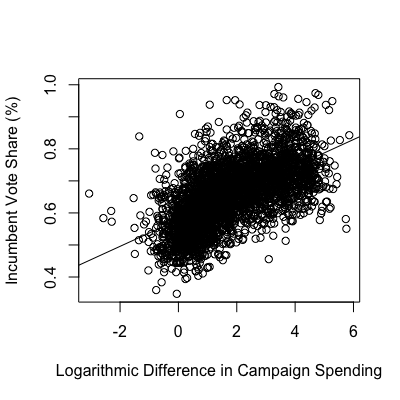
\includegraphics[width=.5\textwidth]{./PS3_Graph_1.png}
		\end{figure}
		The scatterplot and regression line are shown in Figure 1.
	 	\vspace{.7cm}
		\item Save the residuals of the model in a separate object.	
		\lstinputlisting[language=R, firstline=68, lastline=71]{PS3.R}  
		\vspace{.7cm}
		\item Write the prediction equation.
		Prediction Equation: ${\hat{Y} = 0.5970321 + 0.041666X}$
	\end{enumerate}
	
\newpage

\section*{Question 2 (20 points)}
\noindent We are interested in knowing how the difference between incumbent and challenger's spending and the vote share of the presidential candidate of the incumbent's party are related.	\vspace{.25cm}
	\begin{enumerate}
		\item Run a regression where the outcome variable is \texttt{presvote} and the explanatory variable is \texttt{difflog}.
		\lstinputlisting[language=R, firstline=83, lastline=88]{PS3.R}  
		\begin{verbatim}
		Residuals:
     Min       1Q   Median       3Q      Max 
-0.32196 -0.07407 -0.00102  0.07151  0.42743 

Coefficients:
            Estimate Std. Error t value Pr(>|t|)    
(Intercept) 0.507583   0.003161  160.60   <2e-16 ***
difflog     0.023837   0.001359   17.54   <2e-16 ***
Signif. codes:  0 ‘***’ 0.001 ‘**’ 0.01 ‘*’ 0.05 ‘.’ 0.1 ‘ ’ 1

Residual standard error: 0.1104 on 3191 degrees of freedom
Multiple R-squared:  0.08795,	Adjusted R-squared:  0.08767 
F-statistic: 307.7 on 1 and 3191 DF,  p-value: < 2.2e-16
		\end{verbatim}
		\vspace{.1cm}
		\item Make a scatterplot of the two variables and add the regression line. 	
		\lstinputlisting[language=R, firstline=101, lastline=106]{PS3.R}  
		\begin{figure}[h!]
			\caption{\footnotesize{Difference in Campaign Spending vs. Vote Share of Candidate of Incumbent Party}}
			\vspace{.001cm}
			\centering
			\label{fig:graph2}
			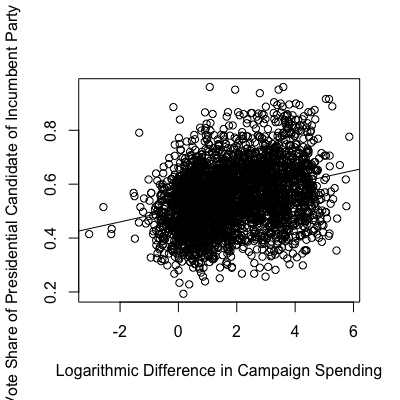
\includegraphics[width=.5\textwidth]{./PS3_Graph_2.png}
		\end{figure}
		The scatterplot and regression line are shown in Figure 2.
		\vspace{.1cm}
		\item Save the residuals of the model in a separate object.
		\lstinputlisting[language=R, firstline=108, lastline=111]{PS3.R}  
		\vspace{.3cm}
		\item Write the prediction equation.
		Prediction Equation: ${\hat{Y} = 0.507583 + 0.023837X}$
	\end{enumerate}
	
	\newpage	
\section*{Question 3 (20 points)}

\noindent We are interested in knowing how the vote share of the presidential candidate of the incumbent's party is associated with the incumbent's electoral success.
	\vspace{.25cm}
	\begin{enumerate}
		\item Run a regression where the outcome variable is \texttt{voteshare} and the explanatory variable is \texttt{presvote}.
			\lstinputlisting[language=R, firstline=122, lastline=127]{PS3.R}  
			\begin{verbatim}
Residuals:
     Min       1Q   Median       3Q      Max 
-0.27330 -0.05888  0.00394  0.06148  0.41365 

Coefficients:
            Estimate Std. Error t value Pr(>|t|)    
(Intercept) 0.441330   0.007599   58.08   <2e-16 ***
presvote    0.388018   0.013493   28.76   <2e-16 ***
---
Signif. codes:  0 ‘***’ 0.001 ‘**’ 0.01 ‘*’ 0.05 ‘.’ 0.1 ‘ ’ 1

Residual standard error: 0.08815 on 3191 degrees of freedom
Multiple R-squared:  0.2058,	Adjusted R-squared:  0.2056 
F-statistic:   827 on 1 and 3191 DF,  p-value: < 2.2e-16
			\end{verbatim}
			\vspace{.5cm}
		\item Make a scatterplot of the two variables and add the regression line. 
				\lstinputlisting[language=R, firstline=140, lastline=145]{PS3.R}  
		\begin{figure}[h!]
			\caption{\footnotesize{Vote Share of Candidate of Incumbent Party vs. Incumbent's Electoral Success}}
			\vspace{.001cm}
			\centering
			\label{fig:graph3}
			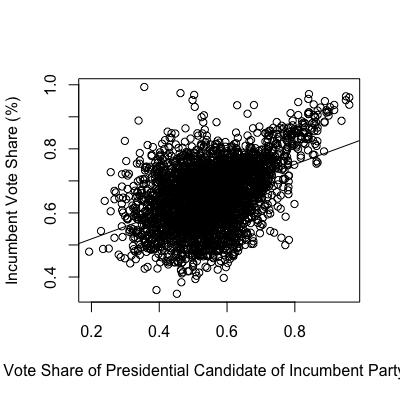
\includegraphics[width=.5\textwidth]{./PS3_Graph_3.png}
		\end{figure}
		The scatterplot and regression line are shown in Figure 3.
			\vspace{.5cm}
		\item Write the prediction equation.
		Prediction Equation: ${\hat{Y} = 0.441330 + 0.388018X}$
	\end{enumerate}
	

\newpage	
\section*{Question 4 (20 points)}
\noindent The residuals from part (a) tell us how much of the variation in \texttt{voteshare} is $not$ explained by the difference in spending between incumbent and challenger. The residuals in part (b) tell us how much of the variation in \texttt{presvote} is $not$ explained by the difference in spending between incumbent and challenger in the district.
	\begin{enumerate}
		\item Run a regression where the outcome variable is the residuals from Question 1 and the explanatory variable is the residuals from Question 2.
		\lstinputlisting[language=R, firstline=157, lastline=162]{PS3.R}  
\begin{verbatim}
Residuals:
     Min       1Q   Median       3Q      Max 
-0.25928 -0.04737 -0.00121  0.04618  0.33126 

Coefficients:
              Estimate Std. Error t value Pr(>|t|)    
(Intercept) -4.860e-18  1.299e-03    0.00        1    
residual2    2.569e-01  1.176e-02   21.84   <2e-16 ***
---
Signif. codes:  0 ‘***’ 0.001 ‘**’ 0.01 ‘*’ 0.05 ‘.’ 0.1 ‘ ’ 1

Residual standard error: 0.07338 on 3191 degrees of freedom
Multiple R-squared:   0.13,	Adjusted R-squared:  0.1298 
F-statistic:   477 on 1 and 3191 DF,  p-value: < 2.2e-16
\end{verbatim}
		\vspace{.6cm}
		\item Make a scatterplot of the two residuals and add the regression line. 
		\lstinputlisting[language=R, firstline=175, lastline=180]{PS3.R}  
		\begin{figure}[h!]
		\caption{\footnotesize{Question 2 Residuals vs. Question 1 Residuals}}
		\vspace{.001cm}
		\centering
		\label{fig:graph4}
		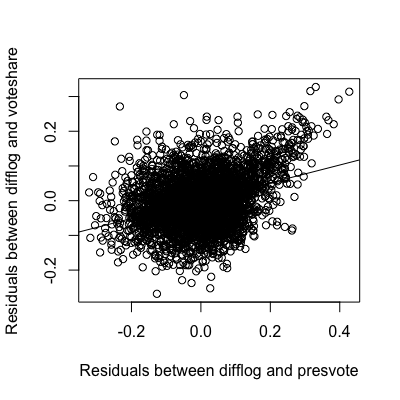
\includegraphics[width=.5\textwidth]{./PS3_Graph_4.png}
		\end{figure}
		The scatterplot and regression line are shown in Figure 4.
		\vspace{.6cm}
		\item Write the prediction equation.
		Prediction Equation: ${\hat{Y} = -4.860*10^-18 + 0.2569X}$
	\end{enumerate}
	
	\newpage	

\section*{Question 5 (20 points)}
\noindent What if the incumbent's vote share is affected by both the president's popularity and the difference in spending between incumbent and challenger? 
	\begin{enumerate}
		\item Run a regression where the outcome variable is the incumbent's \texttt{voteshare} and the explanatory variables are \texttt{difflog} and \texttt{presvote}.
		\lstinputlisting[language=R, firstline=191, lastline=196]{PS3.R}  
\begin{verbatim}
Residuals:
     Min       1Q   Median       3Q      Max 
-0.25928 -0.04737 -0.00121  0.04618  0.33126 

Coefficients:
             Estimate Std. Error t value Pr(>|t|)    
(Intercept) 0.4486442  0.0063297   70.88   <2e-16 ***
difflog     0.0355431  0.0009455   37.59   <2e-16 ***
presvote    0.2568770  0.0117637   21.84   <2e-16 ***
---
Signif. codes:  0 ‘***’ 0.001 ‘**’ 0.01 ‘*’ 0.05 ‘.’ 0.1 ‘ ’ 1

Residual standard error: 0.07339 on 3190 degrees of freedom
Multiple R-squared:  0.4496,	Adjusted R-squared:  0.4493 
F-statistic:  1303 on 2 and 3190 DF,  p-value: < 2.2e-16
\end{verbatim}
\vspace{.6cm}
		\item Write the prediction equation.			\vspace{.5cm}
		Prediction Equation: ${\hat{Y} = 0.4486442 + 0.0355431X_1 + 0.2568770X_2}$

		\item What is it in this output that is identical to the output in Question 4? Why do you think this is the case?
	% My Reflections: The beta_1 in question 4 is identical to the beta_2 in question 5 i.e. the coefficient for presvote as well as the standard error, t statistic, and p-value.
	%This similarity is likely question 4 involved variation in presvote (its variation not explained by difflog) i.e. residual from question 2 that was explained by variation in voteshare (its variation not explained by difflog) i.e. residual from question 1. This isolated the impact of presvote on voteshare from any influence of difflog.
	%Question 5 similarly accounts for voteshare's variation explained by presvote while holding difflog constant. Finding this beta_2 in question 5 requires a similar process of holding difflog constant, so their values are similar.
	
	% Also, the residuals and residual standard error are similar, the only difference explained by difference in degrees of freedom from adding an extra variable in question 5. Question 4 calculates the difference between how the residuals in variation in voteshare explained by difflog predict the residuals in presvote explained by diff log versus how the residuals in presvote explained by difflog actually are. This is equivalent to, in question 5, calculating the difference in predicted voteshare from presvote, difflog, and their predicted coefficients versus the actual observed voteshare.
			\vspace{.5cm}
		(Reflection hidden)
	%	\item Reflect on your finding. Don't write anything. Just think about it.
	\end{enumerate}




\end{document}
